\documentclass[letterpaper,11pt]{article}
\usepackage[margin=1in,dvips]{geometry}
\usepackage{graphicx,float,psfrag,amsmath,amsthm,amssymb}
\usepackage{natbib}
\usepackage{enumitem}
\usepackage{url,color,booktabs,verbatim}
%\usepackage[hidelinks]{hyperref}
\usepackage[colorlinks=true,allcolors=blue,linktoc=all,hyperindex=true]{hyperref}

\usepackage{microtype}
\DisableLigatures{encoding = *, family = * }

%\usepackage{titlesec}
\newcommand{\sectionbreak}{\clearpage}

\bibpunct[, ]{(}{)}{;}{a}{,}{,} % Should be the natbib default but it isn't!

\title{\Huge \textbf{Optical Flow}}

\author{
  \Large Jacob Rafati\\ \texttt{jrafatiheravi@ucmerced.edu}\\
  \\  Electrical Engineering and Computers Science\\  
   University of California, Merced
}

\begin{document}

\maketitle

\tableofcontents

\section*{Abstract}
Two-dimensional image motion is the projection of the three-dimensional motion of objects, relative to the viewer, onto its image plane. Temporal sequences of images allow the estimation of projected 2D image motion as image velocities or discrete image displacements. These are usually
called the \emph{optical flow field}. Optical flow is a reliable approximation to two-dimensional image motion and it may then be used to recover the three-dimensional motion through assumptions concerning the structure of optical flow field. Optical flow may also be used in many application such as pedestrian detection and video processing. In this paper, I will introduce the two prominent \emph{differential methods} for computing \emph{optical flow}: \emph{global method} and \emph{local method}. 

\subsection*{Keywords:} Optical flow, Image velocity field, Differential methods, Computer vision, Motion detection, Local method, Global method.

\section{Introduction} 
\label{sec:introduction}
Optical flow is the pattern of apparent motion of objects, surfaces, and edges in a visual scene caused by the relative motion between an observer and a scene \citep{Horn:Schunck:1981}. The concept of optical flow was introduced by the American psychologist James J. Gibson in the 1940s to describe the visual stimulus provided to animals moving through the world \citep{Gibson:1979}. Gibson stressed the importance of optical flow for accordance perception, the ability to discern possibilities for action within the environment. The role of optical flow have been demonstrated further in the literature for perception of movement by the observer in the world, perception of the shape, distance and movement of objects in the environment, and the control of locomotion. There are many applications for optical flow including: image processing, computer graphics and games, analyzing and predicting ocean currents, action recognition, particle image velocimetry, dense structure from motion, estimation of camera motion, pedestrian detection, object tracking, video compression, video denoising and so on. 

Optical flow can arise from relative motion of objects and the viewer. Therefore, optical flow can give important information about the spatial arrangement of the objects viewed and the rate of change \citep{Horn:Schunck:1981}.  Discontinuities in the optical flow can help in segmenting images into regions that correspond to different objects. The optical flow methods attempt to address the problem of recovering the motions of objects relative to the viewer. Sequences of ordered images allow the estimation of motion as either instantaneous image velocities or discrete image displacements. 

In this report, I will first introduce the definition of optical flow field and the difference with motion field and optical flow field in section \ref{sec:optical-flow}. I will briefly introduce different optical flow methods in \ref{sub:summary}. In section \ref{sec:diff-methods}, I will introduce the two class of the \emph{differential method} with more detail, a \emph{global method} in \ref{sec:Horn-Schunck} and a \emph{local method} in \ref{sec:Lucas-Kanade}. The report, slides, Matlab and Python demo on \emph{differntial methods} is available to download in \texttt{https://github.com/root-master/optical-flow}.

\section{Optical Flow Methods}
\label{sec:optical-flow}
Optical flow is the distribution of apparent velocities or movement of brightness patterns in an image. Optical flow can arise from relative motion of objects and the viewer. Therefore, optical flow can give important information about the spatial arrangement of the objects viewed and the rate of change \citep{Horn:Schunck:1981}. Discontinuities in the optical flow can help in segmenting images into regions that correspond to different objects. The optical flow methods attempt to address the problem of recovering the motions of objects relative to the viewer. 
\subsection{Optical flow field vs. Motion field}
The interpretation of intensity variation as pure relative motion is restrictive because velocity is a geometric quantity independent from illumination conditions Hence estimating optical flow from intensity variation only approximates image motion Conditions which make optical flow different from image motion include the absence of texture in which case optical flow is null and when the true motion field violates the brightness consistency model used for its approximation. Uniform scene illumination and Lambertian surface reflectance are either explicitly or implicitly assumed in most current optical flow methods which use some form of the brightness consistency assumption Highlights shadows variable illumination and surface translucency are phenomena violating the assumption and have only been studied to a limited extent.
Optical flow are a class of methods that are trying to find the velocity field between consecutive frames. But they are different from the \emph{motion filed}. Motion field is a velocity field that is a 2D motion field representing the projection of the 3D motion of points in the scene onto the image plane (Fig. \ref{grf:motion-field}). Optical flow methods are computing the velocity field by the difference between two consecutive frames (Fig. \ref{grf:optical-flow-ball}). 5 In the optical flow problem, the intensity of the frame images $I(x,y,t)$ is provided for any pixel location $(x,y)$ and time $t$ and the velocity filed of pixels (or a group of pixels) are required to compute (Fig. \ref{grf:army-flow}). Consequently, optical flow field is not necessarily equal to the motion field. There are few examples that highlights this concept. See Fig. \ref{grf:motion-flow-vs-optical-flow} for three examples where the motion field and the optical flow field is totally different. 

\begin{figure}[ht!]
	\centering
	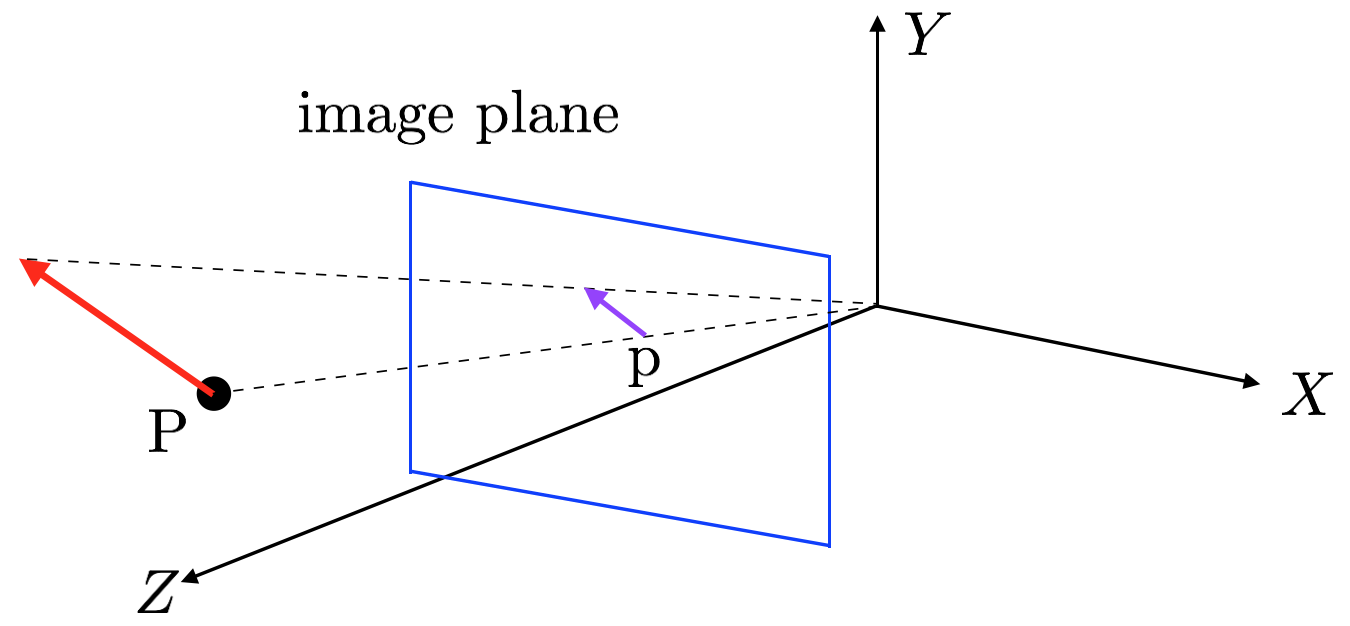
\includegraphics[width=.7\textwidth]{grf/motion-field.png}
	\caption{\emph{Motion Field} is 2D motion field representing the projection of the 3D motion of points in the scene onto the image plane.}
	\label{grf:motion-field}
\end{figure}

\begin{figure*}[hb!]
	\centering
	\begin{tabular}{cc} 
		(a) & (b) \\
		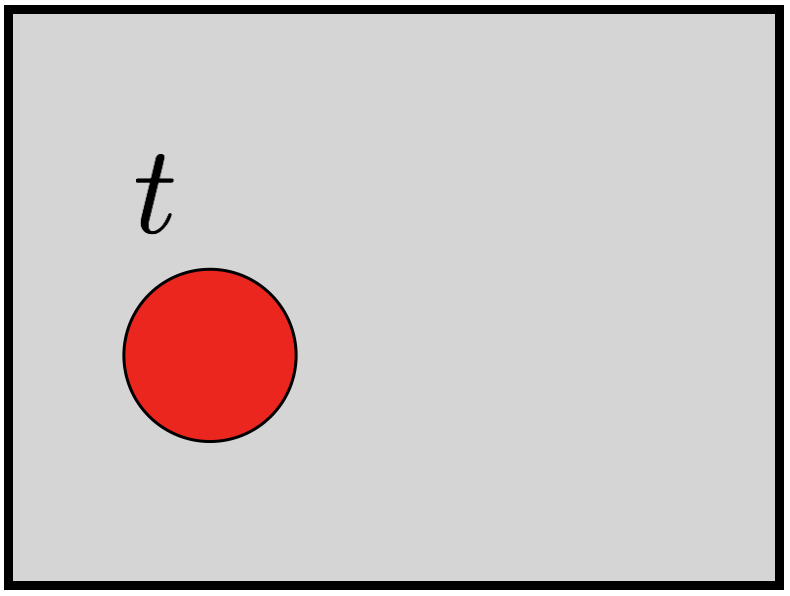
\includegraphics[width=.45\textwidth]{grf/optical-flow-ball-1.png} &
		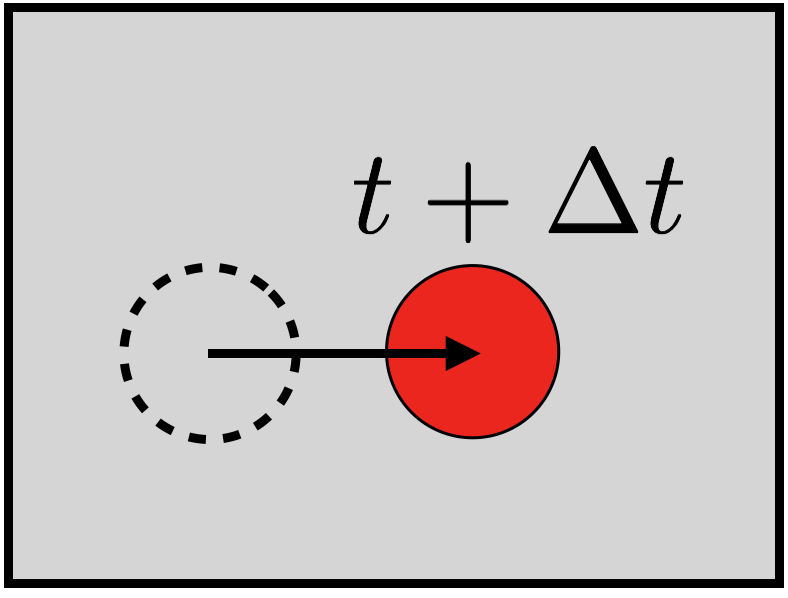
\includegraphics[width=.45\textwidth]{grf/optical-flow-ball-2.png} 
	\end{tabular}
	\caption{Optical flow is 2D velocity field describing the apparent motion of image objects between two consecutive frames. (a): Frame at time $t$. The red object in $(x,y)$ moves towards right side of frame. (b): Frame at time $t+\Delta t$. The red object moved towards right side of the frame to $(x+\Delta x , y + \Delta y)$. The arrow is the optical flow vector between these two frames.}
	\label{grf:optical-flow-ball}
\end{figure*}
  
\begin{figure*}[hbt!]
	\centering
	\begin{tabular}{cc} 
		(a) & (b) \\
		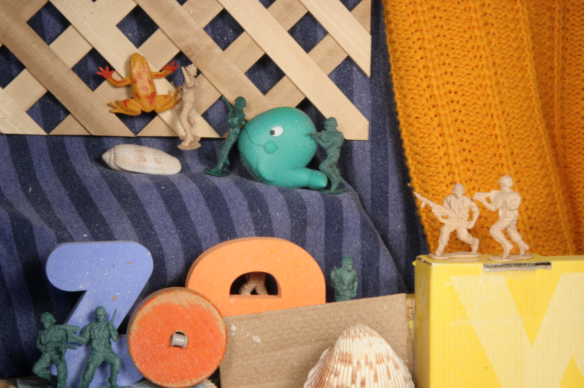
\includegraphics[width=.45\textwidth]{grf/army1.png} &
		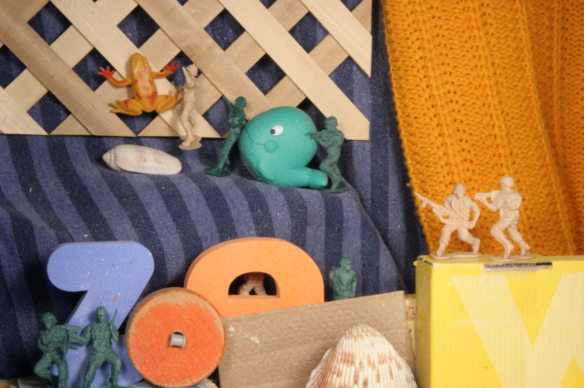
\includegraphics[width=.45\textwidth]{grf/army2.png} \vspace{1cm}\\ 
		(c) & (d) \\
		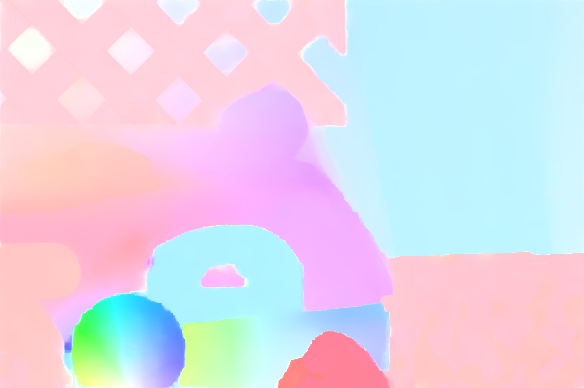
\includegraphics[width=.45\textwidth]{grf/army-flow.png} &
		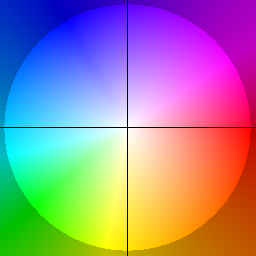
\includegraphics[width=.2\textwidth]{grf/colorwheel.png} 
	\end{tabular}
	\caption{A classical optical flow example (army and rubber whale). (a) Frame at time $t$. (b): Frame at time $t+\Delta t$. (c) Optical flow velocity vector field. (d) Optical flow color wheel: the colors represent the direction of flow and the saturation represent magnitude of optical flow velocity vector.}
	\label{grf:army-flow}
\end{figure*}

\begin{figure*}[hbt!]
	\centering
	\begin{tabular}{ccc} 
		(a) & (b) & (c)\\
		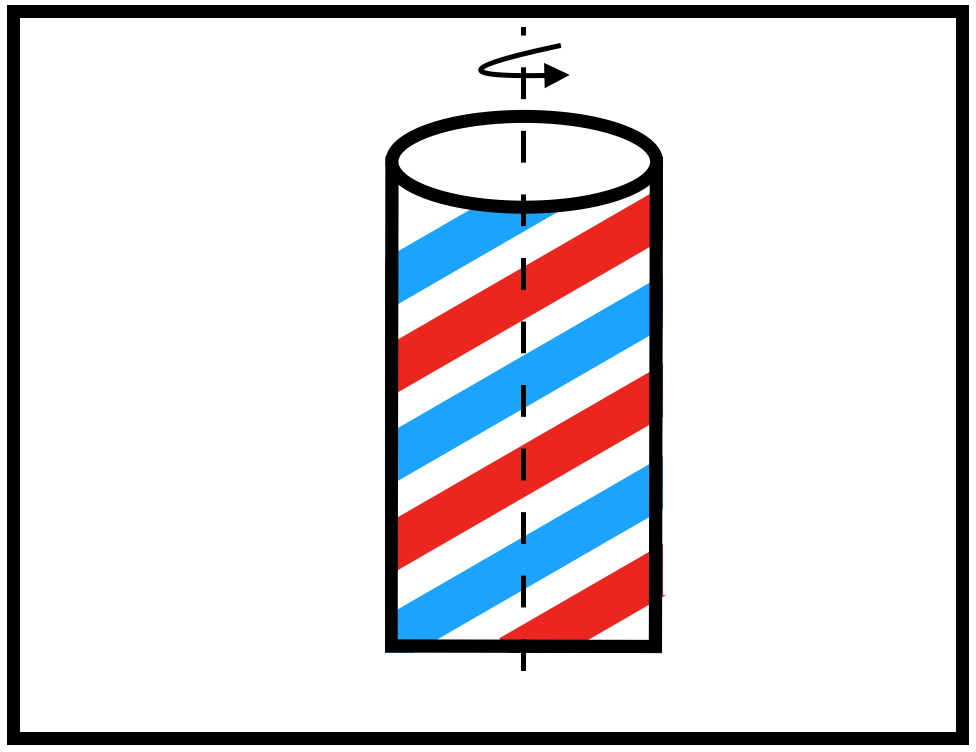
\includegraphics[width=.3\textwidth]{grf/barber-pole.png} &
		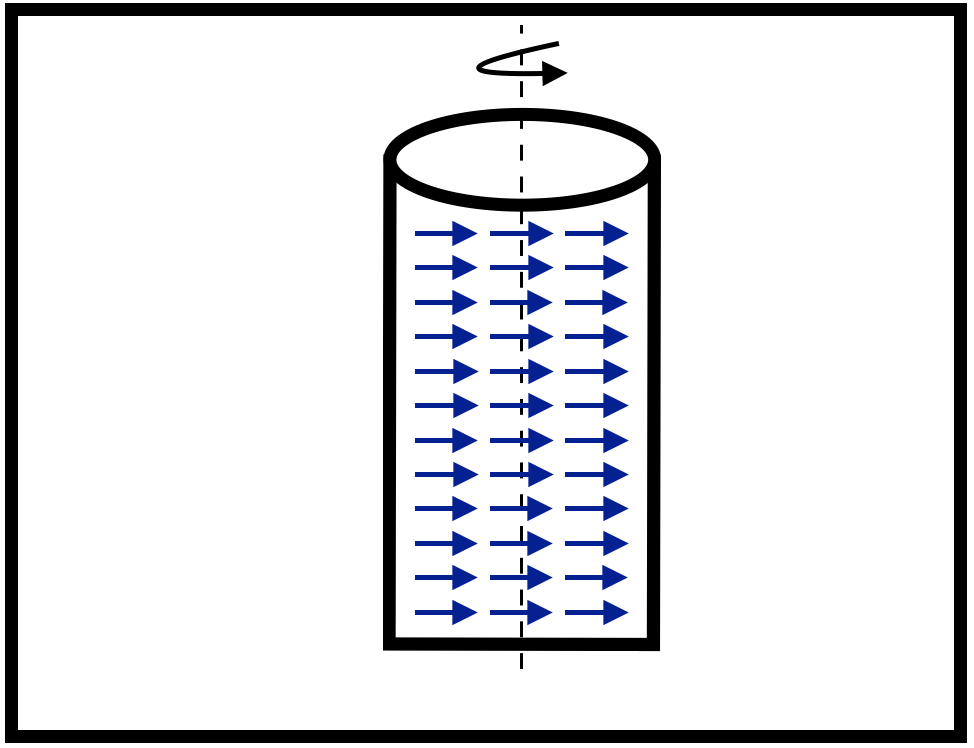
\includegraphics[width=.3\textwidth]{grf/barber-pole-motion-field.png} &
		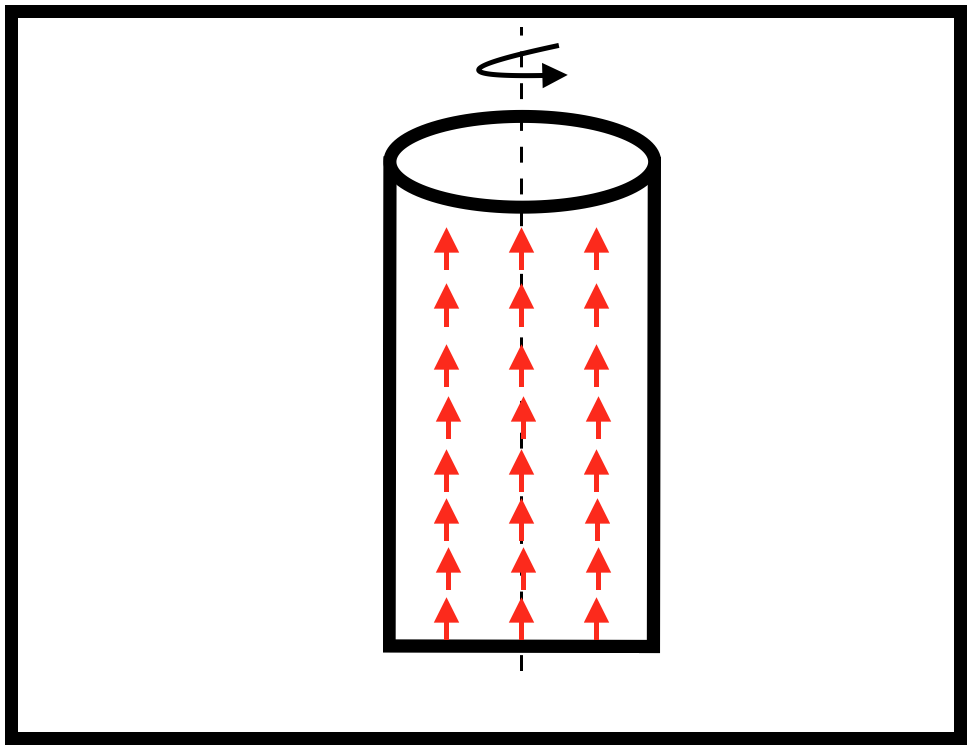
\includegraphics[width=.3\textwidth]{grf/barber-pole-optical-flow.png}
		\vspace{0.5cm}\\ 
		(d) & (e) & (f) \\
		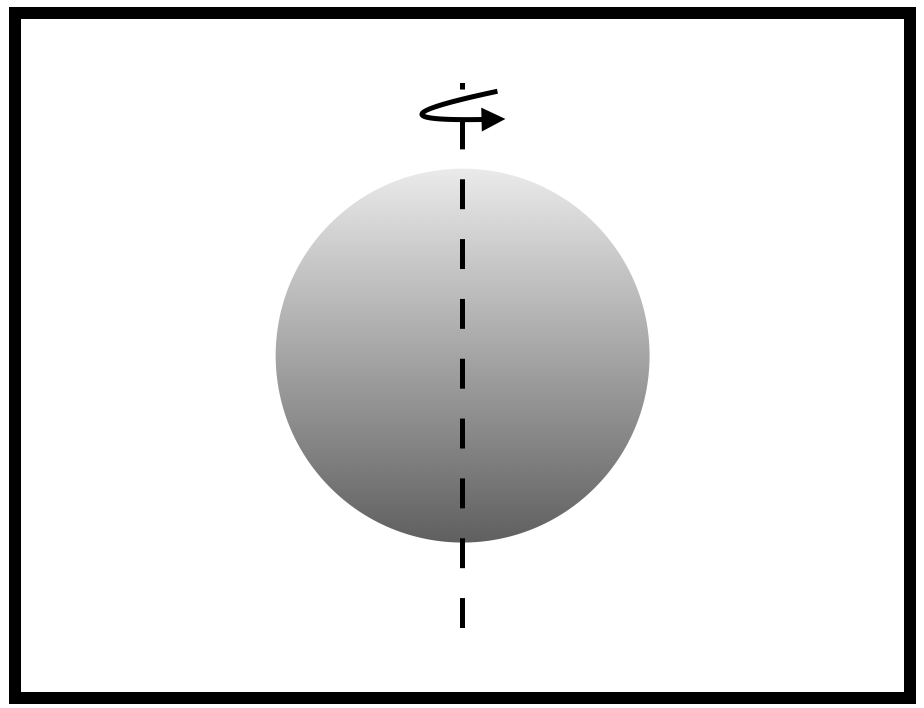
\includegraphics[width=.3\textwidth]{grf/lambertian-sphere.png} &
		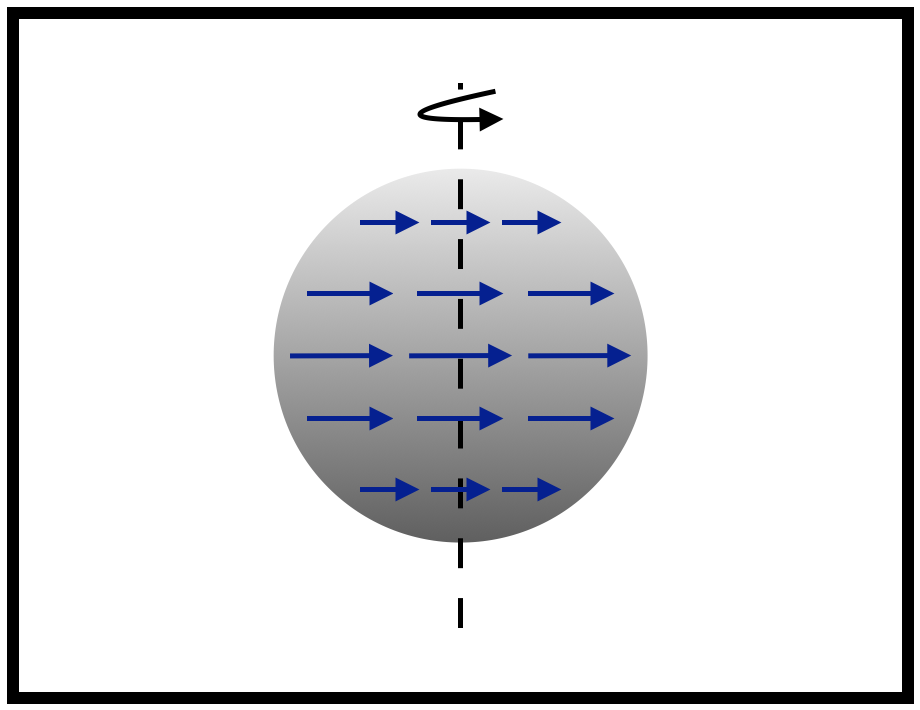
\includegraphics[width=.3\textwidth]{grf/lambertian-sphere-motion-field.png} &
		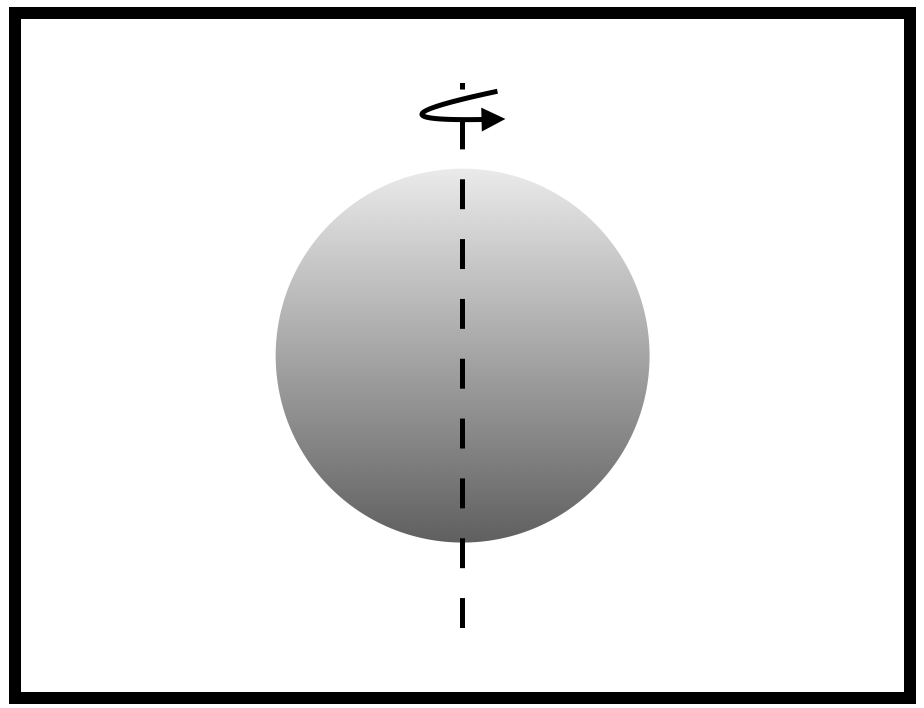
\includegraphics[width=.3\textwidth]{grf/lambertian-sphere-optical-flow.png}
		\vspace{0.5cm}\\ 
		(g) & (h) & (i) \\
		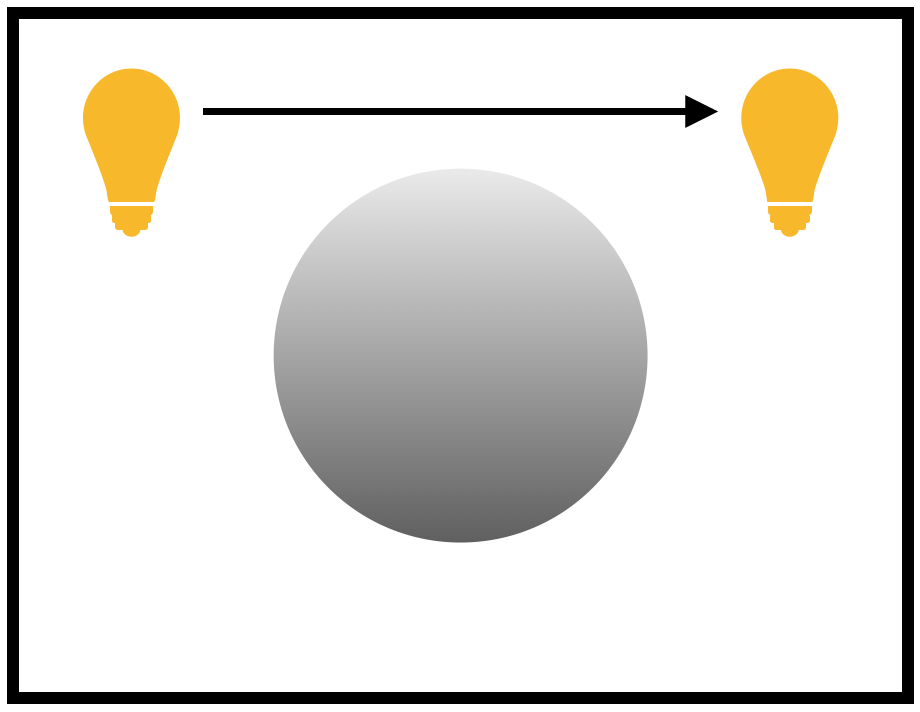
\includegraphics[width=.3\textwidth]{grf/stationary-lambertian-sphere.png} &
		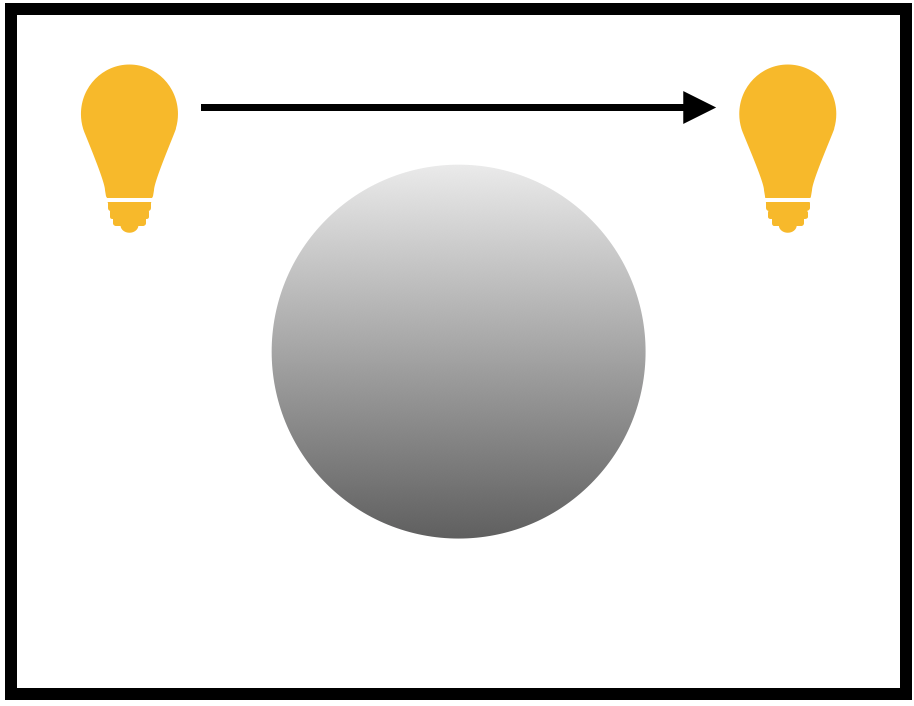
\includegraphics[width=.3\textwidth]{grf/stationary-lambertian-sphere-motion-field.png} &
		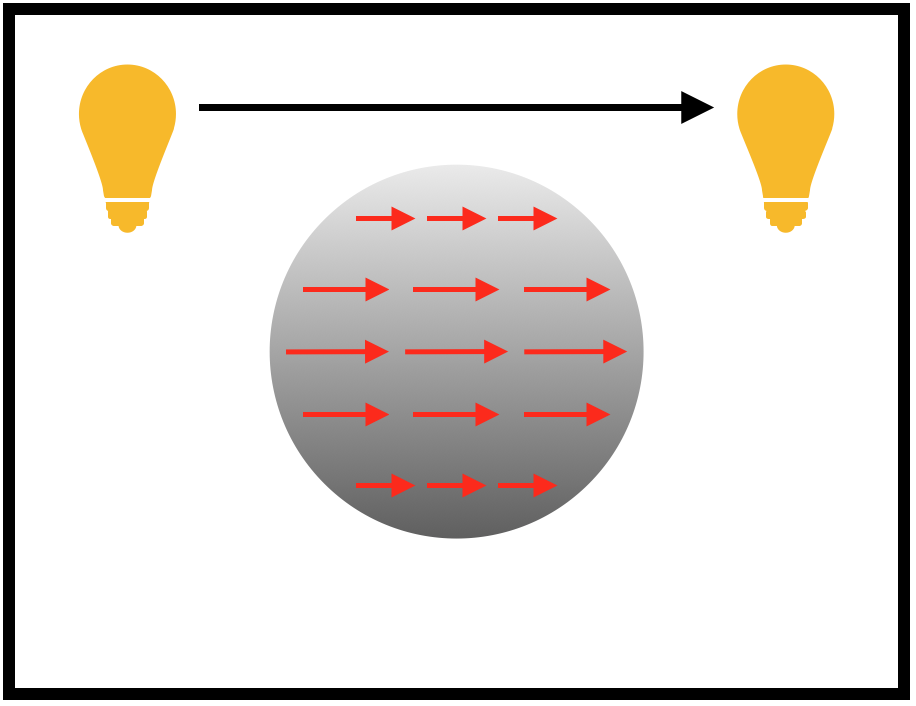
\includegraphics[width=.3\textwidth]{grf/stationary-lambertian-sphere-optical-flow.png}
	\end{tabular}
	\caption{(a) Barber pole illusion: a clolored pole spinning around the cylinder axis. (b) Motion field. (c) Optical flow field. (d) Lambertian (matte) sphere spinning around $z$ axis. (e) Motion field is not zero. (f) Optical flow field is zero. (g) Stationary Lambertian sphere. The light source is moving. (h) Motion field is zero. (i) Optical flow field is not zero. }
	\label{grf:motion-flow-vs-optical-flow}
\end{figure*}

Theoretically researchers believe that optical flow as an approximation to image motion largely determines the lower bound
on accuracy \citep{Beauchemin:1995}. Although examples of Fig. \ref{grf:motion-flow-vs-optical-flow} show that optical flow could not capture the motion field, in practice we can assume that if the displacement is small, oftentimes the optical flow is a good approximation for the motion field. 

\subsection{Optical flow constraint equation}
The optical flow methods attempt to calculate the motion between two image frames which are taken at times $t$ and $t + \Delta t$. Consider a 2D dimensional image, and a pixel at location $\mathbf{x} = (x,y)$ and time $t$ with intensity $I(x,y,t)$. This local image region has a spacial displacement of $\Delta \mathbf{x} = (\Delta x, \Delta y)$ after time $\Delta t$ between two consequent image frames (Fig. \ref{grf:optical-flow-ball}). The initial hypothesis in measuring image motion is that the intensity structures of local time-varying image regions are approximately constant under motion for at least a short duration \citep{Beauchemin:1995,Horn:Schunck:1981}. Formally
\begin{align}
I(x,y,t) \approx I(x + \Delta x, y + \Delta y, t + \Delta t).
\label{eq:intensity-cond}
\end{align}

The \emph{differential methods} are based on local Taylor series approximations of the image signal, i.e. they use partial derivatives with respect to the spatial and temporal coordinates. The image domain is therefore assumed to be continuous (or differentiable) in space and time. Expanding the left-hand side of \eqref{eq:intensity-cond} in a Taylor series yields
\begin{align}
I(x,y,t) = I(x,y,t) +  \frac{\partial I}{\partial x} \Delta x + \frac{\partial I}{\partial y} \Delta y + \frac{\partial I}{\partial t} \Delta t + \textrm{O}({\Delta x}^2,{\Delta y}^2,{\Delta t}^2 ),
\label{eq:intensity-taylor}
\end{align}
where subscripts denote partial differentiation. We can ignore the second and higher order terms, which are assumed negligible. Subtracting \eqref{eq:intensity-taylor} on both sides yields 
\begin{align}
\frac{dI}{dt} = \frac{\partial I}{\partial x}  \dot{x} + \frac{\partial I}{\partial y} \dot{y} + \frac{\partial I}{\partial t} = 0, \quad \textrm{or}\quad  \nabla I \cdot \mathbf{v} + I_{,t} = 0,
\label{eq:flow-diff}
\end{align}
where $\nabla I = (I_{,x},I_{,y}) = (\frac{\partial I}{\partial x} ,\frac{\partial I}{\partial y} )$ is the spatial gradient of the intensity, $\mathbf{v} = (u,v) = (\dot{x},\dot{y})$ is the image \emph{velocity field} or \emph{optical flow vector field}. Note that we assume $\Delta t$ is small and $(\Delta x / \Delta t, \Delta y / \Delta t) \approx (\dot{x},\dot{y})$. Equation \eqref{eq:flow-diff} is known as the \emph{optical flow constraint equation}. This is an equation in two unknowns and cannot be solved as such. This constraint is not sufficient to
compute both components of $\mathbf{v}$ as the optical flow constraint equation is ill-posed (Fig. \ref{grf:ill-posed}).
\begin{figure}[ht!]
	\centering
	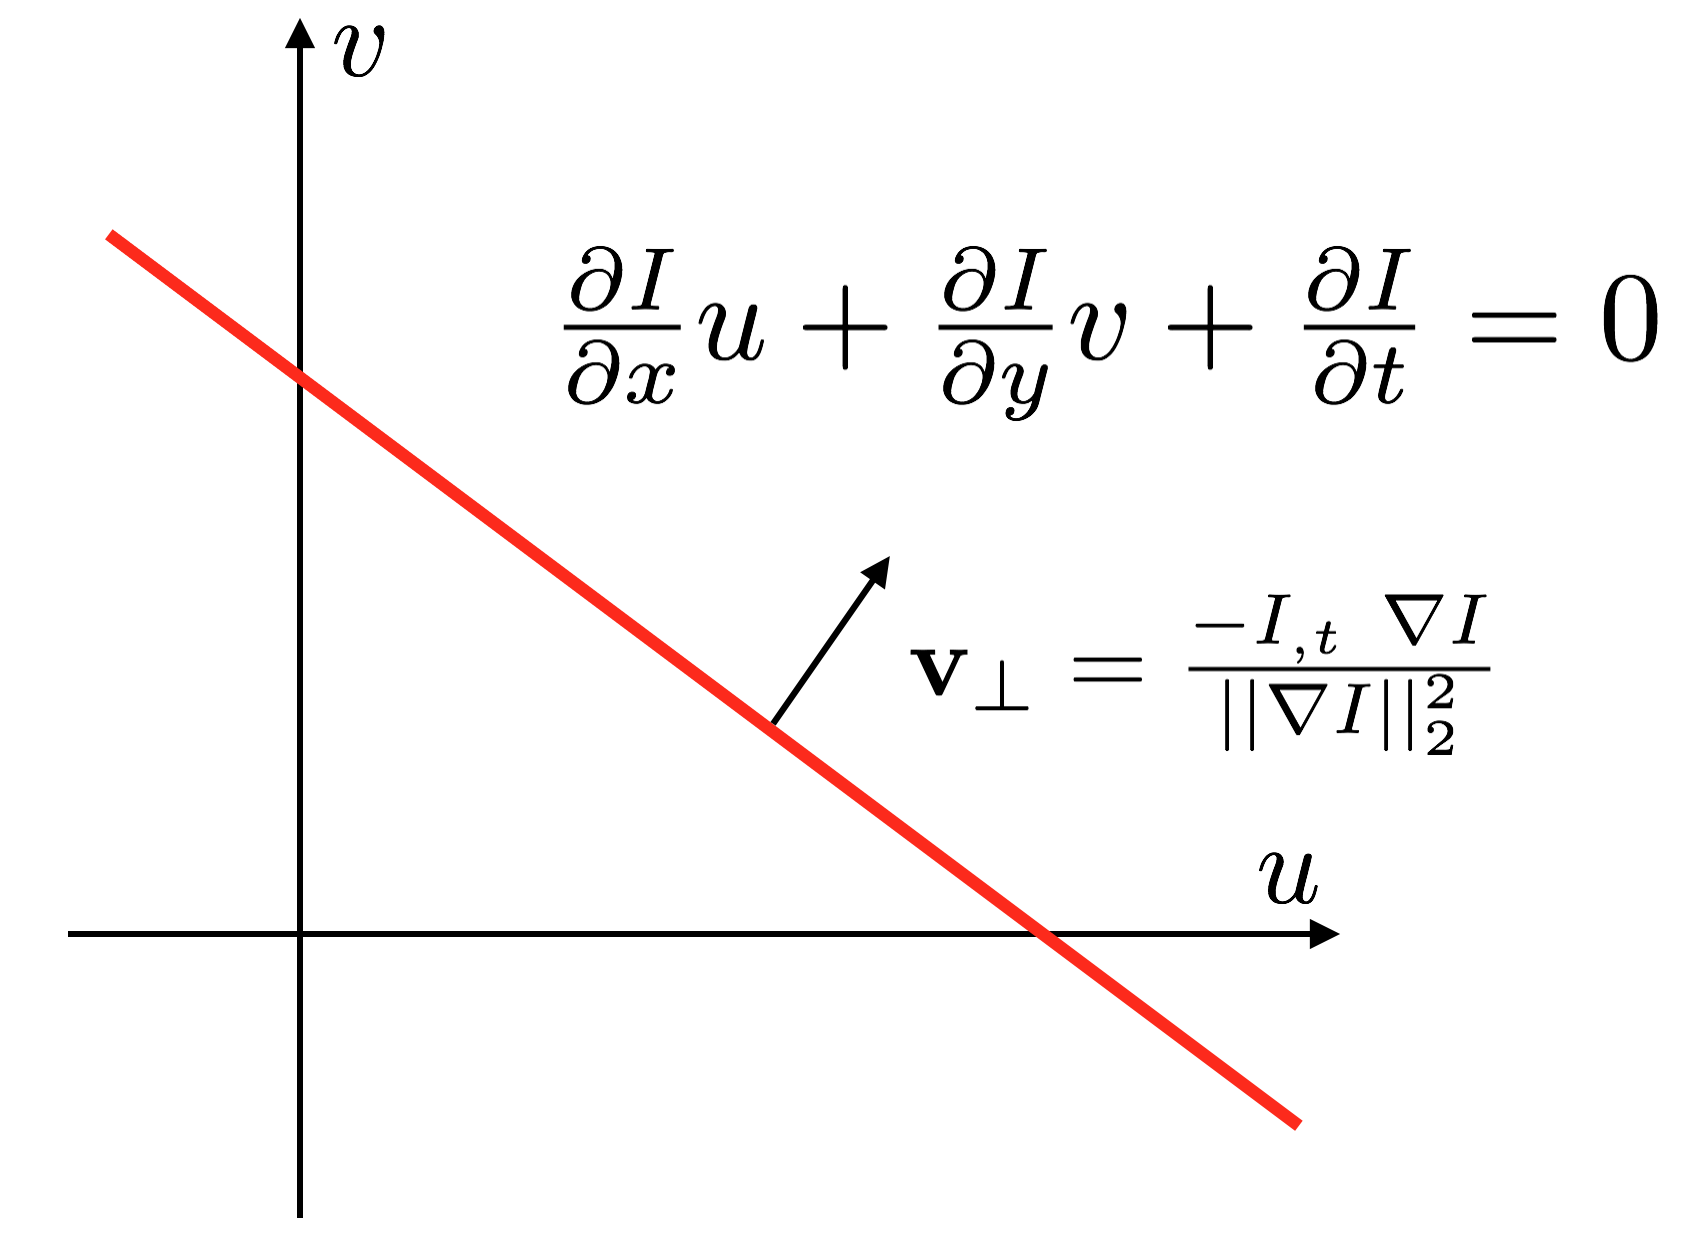
\includegraphics[width=.7\textwidth]{grf/ill-posed.png}
	\caption{\emph{Optical flow constraint equation} is ill-posed since it is not sufficient to
compute both components of $\mathbf{v}$. Only $\mathbf{v_{\perp}}$ the motion component in the direction of the local gradient of the image intensity
function can be estimated.}
	\label{grf:ill-posed}
\end{figure}
That is to say, only $\mathbf{v_{\perp}}$ the motion component in the direction of the local gradient of the image intensity
function, may be estimated
\begin{align}
\mathbf{v_{\perp}} = \frac{- I_t ~\nabla I}{|| \nabla I ||_2^2}.
\label{eq:normal-v}
\end{align}
This phenomenon is known as the aperture problem and only at image
locations where there is sufficient intensity structure (or Gaussian curvature) can the motion be fully estimated with the use of the optical flow constraint equation \citep{Beauchemin:1995}. To find the optical flow another set of equations is needed, given by some additional constraint. All optical flow methods introduce additional conditions for estimating the actual flow.

\subsection{Summary of methods}
\label{sub:summary}
There exist numerous computational models for estimating image velocity which can be classified into the following main groups
\begin{description}
\item[\bf{Differential Methods}.] Differential techniques compute image velocity from spatio-temporal derivatives of image intensities The image domain is therefore assumed to be continuous or differentiable in space and
time. Global and local first and second order methods based on \eqref{eq:flow-diff} can be used to compute optical fow. \emph{Global methods} use \eqref{eq:flow-diff} and an additional global constraint usually a smoothness
regularization term to compute dense optical flow over large image regions \citep{Beauchemin:1995,Horn:Schunck:1981}. \emph{Local methods} use normal velocity information in local neighborhood to perform a least squares minimization to find the best fit for $\mathbf{v (\mathbf{x}) } = (u(\mathbf{x}),v(\mathbf{x}))$ \citep{Lucas:Kanade:1981}. More detail on this approach is provided in section \ref{sec:diff-methods}. For additional detail see \citep{Beauchemin:1995}.
\item[\bf{Frequency-Based Methods}.] A second class of optical flow techniques is based on the use of velocity-tuned filters.
These techniques use orientation sensitive filters in the Fourier domain of time-varying images. For more detail see \citep{Beauchemin:1995}.
\item[\bf{Correlation-Based Methods}.] Numerical differentiation is sometimes impractical because of small temporal support (only a few frames) or poor signal-to-noise ratio. In these cases, differential or frequency approaches may not be appropriate and it is natural to consider matching methods. Correlation-based matching approaches are less sensitive to these problems: they do not rely on the presence of significant image features and variable correlation window sizes can be used near occlusion boundaries to handle multiple
motions. These approaches define displacement (which is an approximation to velocity) as a shift that yields the best fit between contiguous time-varying image regions. For more detail see \citep{Beauchemin:1995}. For more detail see \citep{Beauchemin:1995}.
\item[\bf{Multiple Motion Methods}.] Many phenomena can cause multiple image motions. Among them, occlusion and transparency are important in terms of their occurrence and significance in realistic imagery. This framework consists of the minimization of a functional that expresses the various assumptions made about image motion. For more detail see \citep{Beauchemin:1995}.
\item[\bf{Temporal Refinement Methods}.] Most of the optical flow methods do not incorporate
motion estimates from previous calculations within an image sequence being acquired: given two or more images, optical flow is computed only for one of the images. Temporal Refinement Methods use incremental computation of optical flow. Temporal continuity allows prediction of the next image velocity, assuming uniform acceleration.For more detail see \citep{Beauchemin:1995}. 
\item[\bf{Supervised methods with convolutional neural network}.]  Recently, CNNs are being used to solve
the optical flow estimation problem as a supervised learning task. Supervised learning require large data with true labels. To train the optical flow network, \citep{FlowNet:2015} generated a large synthetic dataset. 
\end{description}

\section{Differential Methods}
\label{sec:diff-methods}
Differential techniques compute image velocity filed from spatio-temporal derivatives of image intensities. The image domain
is therefore assumed to be continuous (or differentiable) in space and time. Global and local first and second-order methods
based on Equation \eqref{eq:flow-diff} can be used to compute optical flow. Global methods use
\eqref{eq:flow-diff} and an additional global constraint, usually a smoothness regularization term, to compute dense optical flows over
large image regions. Local methods use normal velocity information in local neighborhoods to perform a least squares minimization to find the best fit for $\mathbf{v}$.
The size of the neighborhood for obtaining a velocity estimate determines whether each individual technique is local or global. A surface or contour model may also be used to integrate normal velocities into full velocity. Large 2D motions may be analyzed in a hierarchical framework, possibly in conjunction with warping methods.

\subsection{A Global Method: Horn-Schunck Algorithm}
\label{sec:Horn-Schunck}
The Horn-Schunck algorithm \citep{Horn:Schunck:1981} assumes smoothness in the flow over the whole image. Thus, it tries to minimize distortions in flow and prefers solutions which show more smoothness.
\subsubsection*{The Smoothness Constraint}
The smoothness constraint is based on the assumption that the neighboring points on the objects have similar velocities and the velocity field of the
brightness patterns in the image varies smoothly almost everywhere. Discontinuities in flow can be expected where one object occludes another. An algorithm based on a smoothness constraint is likely to have difficulties with
occluding edges as a result. One way to express the additional constraint is to minimize the square of the
magnitude of the gradient of the optical flow velocity: 
\begin{align}
|| \nabla u ||^2 = (\frac{\partial u}{\partial x})^2 + (\frac{\partial u}{\partial y})^2, \quad || \nabla v ||^2 = (\frac{\partial v}{\partial x})^2 + (\frac{\partial v}{\partial y})^2.
\label{eq:Horn-smoothness-constraint-gradient}
\end{align}
Another measure of the smoothness of the optical flow field is the sum of the squares of the Laplacians of the $x$- and $y$-components of the flow. The Laplacians of $u$ and $v$ are defined as
\begin{align}
\nabla^2 u = \frac{\partial^2 u}{\partial x^2} + \frac{\partial^2 u}{\partial y^2}, \quad \nabla^2 v = \frac{\partial^2 v}{\partial x^2} + \frac{\partial^2 v}{\partial y^2}.
\label{eq:Horn-smoothness-constraint-Laplacian}
\end{align}
The optical flow constraint equation \eqref{eq:flow-diff} is made in conjunction with a regularization term \eqref{eq:Horn-smoothness-constraint-gradient} to define an error functional over the image domain $D$
\begin{align}
E[(u,v)] = \iint_D \Big \{  (I_{,x} u + I_{,y} v + I_{,t})^2 + \lambda^2 ( || \nabla u ||^2 + ||\nabla v|| ^2 ) \Big \} ~ dx dy,  
\label{eq:Horn:energy-fuctional-gradient}
\end{align}
where $\lambda$ is a regularization constant. Another alternative to form the energy function is using \eqref{eq:Horn-smoothness-constraint-Laplacian} as a smoothness regularization constraint
\begin{align}
E[(u,v)] = \iint_D \Big \{  (I_{,x} u + I_{,y} v + I_{,t})^2 + \lambda^2 ( \nabla^2 u + \nabla^2 v ) \Big \} ~ dx dy.  
\label{eq:Horn:energy-fuctional-laplacian}
\end{align}   
The optical flow can be found by solving the optimization problem over the global energy (error) functional, either \eqref{eq:Horn:energy-fuctional-gradient} or \eqref{eq:Horn:energy-fuctional-laplacian}
\begin{align}
\min_{(u,v)} E[(u,v)].
\label{eq:Horn:optimization}
\end{align}
For the purpose of solving this optimization problem we only consider \eqref{eq:Horn:energy-fuctional-gradient}. This functional can be minimized by solving the associated multi-dimensional Euler-Lagrange equations. These are
\begin{subequations}
\begin{align}
\frac{\partial L}{\partial u} - \frac{\partial}{\partial u}\frac{\partial L}{\partial u_{,x}} - \frac{\partial}{\partial u}\frac{\partial L}{\partial u_{,y}} = 0, \\
\frac{\partial L}{\partial v} - \frac{\partial}{\partial v}\frac{\partial L}{\partial v_{,x}} - \frac{\partial}{\partial v}\frac{\partial L}{\partial v_{,y}} = 0, 
\end{align}
\label{eq:Lagrangian}
\end{subequations}
where $L$ is the integrand of the energy expression from \eqref{eq:Horn:energy-fuctional-gradient}
\begin{align}
L = (I_{,x} u + I_{,y} v + I_{,t})^2 + \lambda^2 ( || \nabla u ||^2 + ||\nabla v|| ^2 ).
\label{eq:Horn:L}
\end{align}
Substituting $L$ from \eqref{eq:Horn:L} into the Euler-Lagrange equations \eqref{eq:Lagrangian} we have
\begin{subequations}
\begin{align}
I_{,x} (I_{,x} u + I_{,y} v + I_{,t}) - \lambda^2 \nabla^2 u &= 0, \\
I_{,y} (I_{,x} u + I_{,y} v + I_{,t}) - \lambda^2 \nabla^2 v &= 0
\end{align}
\label{eq:Horn:Lagrangian}
\end{subequations}
where subscripts again denote partial differentiation and $\nabla^2 = \frac{\partial^2}{\partial x^2} + \frac{\partial^2}{\partial y^2}$ denotes the Laplace operator. In practice the Laplacian is approximated numerically using finite differences, and may be written
\begin{subequations}
\begin{align}
\nabla^2 u(x,y) = \bar{u} (x,y) - u(x,y),\\
\nabla^2 v(x,y) = \bar{v} (x,y) - v(x,y),
\end{align}
\label{eq:laplace-difference-approximation}
\end{subequations}
where $(\bar{u}(x,y),\bar{v}(x,y))$ is a weighted average of $(u(x,y),v(x,y))$ calculated in a neighborhood around the pixel at location $(x,y)$ and can be computed by applying the following filter on $(u,v)$:
\begin{align}
\mathcal{L} = \begin{bmatrix}
\frac{1}{12} & \frac{1}{6} & \frac{1}{12} \\
\frac{1}{6} & -1 & \frac{1}{6} \\
\frac{1}{12} & \frac{1}{6} & \frac{1}{12} 
\end{bmatrix}.
\end{align}
Using the weighted difference method \eqref{eq:laplace-difference-approximation} in \eqref{eq:Horn:Lagrangian} yileds to the linear system 
\begin{align}
\begin{bmatrix}
I_{,x}^2 + \lambda^2 & I_{,x} I_{,y} \\
I_{,x} I_{,y} & I_{,y}^2 + \lambda^2
\end{bmatrix} \begin{bmatrix}
u \\
v
\end{bmatrix} = \begin{bmatrix}
\lambda^2 \bar{u} - I_{,x} I_{,t} \\
\lambda^2 \bar{v} - I_{,y} I_{,t}
\end{bmatrix}
\label{eq:Horn:lagrange-difference-approximation}
\end{align}
which is linear in $u$ and $v$ and may be solved for each pixel in the image. The result is a linear equation in the form of 
\begin{align}
\begin{bmatrix}
    c_{11} & c_{12} & &\textrm{\LARGE0} \\
c_{12}& c_{22} &\ddots &\\   
&  \ddots& \ddots & \\
    \text{\LARGE0}& & & 
\end{bmatrix}
\begin{bmatrix}
u_1\\
v_1\\
\vdots\\
\vdots
\end{bmatrix}
= \begin{bmatrix}
-I_{,x}^{(1)} I_{,t}^{(1)}\\
-I_{,y}^{(1)} I_{,t}^{(1)}\\
\vdots\\
\vdots\\
\end{bmatrix}
\end{align}
where $C = [c_{ij}]$ is a sparse matrix. Apparently, solving this linear equation was challenging for \citep{Horn:Schunck:1981} due to the computational cost, therefore they used the Jacobi iterative method to compute the optical flow for each pixel:
\begin{subequations}
\begin{align}
u^{k+1} = \bar{u}^{k} - \frac{I_{,x} (I_{,x} \bar{u}^{k} + I_{,y} \bar{v}^{k} + I_{,t}) }{\lambda^2 + I_{,x}^2 + I_{,y}^2},\\
v^{k+1} = \bar{v}^{k} - \frac{I_{,y} (I_{,x} \bar{u}^{k} + I_{,y} \bar{v}^{k} + I_{,t}) }{\lambda^2 + I_{,x}^2 + I_{,y}^2},
\end{align}
\end{subequations}
where the superscript $k+1$ denotes the next iteration, which is to be calculated and $k$ is the last calculated result.
\subsubsection*{Assumptions and Properties}
Uniform illumination (at least locally) in the image domain of interest, orthographic projection, and pure translational motion parallel to the scene are conditions that must be met for the brightness constancy assumption $(dI / dt = 0)$ to be satisfied \citep{Beauchemin:1995}.
Advantages of the Horn-Schunck algorithm include that it yields a high density of flow vectors, i.e. the flow information missing in inner parts of homogeneous objects is filled in from the motion boundaries. On the negative side, it is more sensitive to noise than local methods.


\subsection{A Local Method: Lucas-Kanade Algorithm}
\label{sec:Lucas-Kanade}
The Lucas-Kanade optical flow algorithm is a simple technique which can provide an estimate of the movement of \emph{interesting features} in successive
images of a scene. Let's denote the optical flow field by $\mathbf{v} = (u, v)$. Every such ``interesting'' pixel in the scene, obtained by comparing the two consecutive images. Lucas and Kanade use a local constant model for $\mathbf{v} $ which
is solved as a weighted least squares solution to \eqref{eq:flow-diff} \citep{Lucas:Kanade:1981}. Velocity estimates are
computed by solving the minimizing problem
\begin{align}
\min \sum_{\mathbf{x}_i \in R(\mathbf{x})}W(\mathbf{x}_i;\mathbf{x})(\nabla I(\mathbf{x}_i,t) \cdot \mathbf{v} + I_t(\mathbf{x}_i,t))^2,
\label{eq:lucas:canade:optim}
\end{align}
where $R = \{ \mathbf{x}_1,\dots,\mathbf{x}_n \}$ is a spatial neighborhood with a cardinality of $n$ and $W(\mathbf{x})$ is a $n \times n$ diagonal matrix denotes a window function.  In practice it is usually better to give more weight to the pixels that are closer to the central pixel $p$. The Lucas-Kanade method assumes that the displacement of the image contents between two nearby instants (frames) is small and approximately constant within a neighborhood of the point $p$ under consideration. Thus the optical flow equation can be assumed to hold for all pixels within a window centered at $p$. Solutions for $\mathbf{v}$ are obtained in closed form. The local image flow vector $\mathbf{v} = (u,v)$ must satisfy \eqref{eq:flow-diff}
\begin{align}
W S \mathbf{v} = W b,
\label{eq:lucal-kanade-matrix}
\end{align}
where
\begin{align}
S = \begin{bmatrix}
I_{,x}(\mathbf{x}_1) & I_{,y}(\mathbf{x}_1)\\
\vdots & \vdots\\
I_{,x}(\mathbf{x}_i) & I_{,y}(\mathbf{x}_i) \\
\vdots & \vdots\\
I_{,x}(\mathbf{x}_n) & I_{,y}(\mathbf{x}_n) 
\end{bmatrix},  \quad \mathbf{v} = \begin{bmatrix}
u \\
v
\end{bmatrix}, \quad \textrm{and} \quad b = \begin{bmatrix}
-I_{,t}(\mathbf{x}_1) \\
\vdots \\
-I_{,t}(\mathbf{x}_i) \\
\vdots \\
-I_{,t}(\mathbf{x}_n) 
\end{bmatrix}
\end{align} 
Equation \eqref{eq:lucal-kanade-matrix} cannot be solved exactly (in the general case). The Least Squares solution is found by multiplying the equation \eqref{eq:lucal-kanade-matrix} by $S^T$
\begin{align}
S^T W S \mathbf{v} = S^T W b.
\label{eq:lucas-kanade-leastsqaure}
\end{align} 
If $S^T S$ is invertable, $\mathbf{v}$ can be found as
\begin{align}
\mathbf{v} = (S^T W S)^{-1} S^T W b.
\label{eq:lucas-kanade-compact-solution}
\end{align}
That is, it computes
\begin{equation}
\begin{bmatrix}
u \\
~\\
\\
v
\end{bmatrix} = 
\begin{bmatrix}
\sum\limits_{\mathbf{x}_i \in R} W_{ii} I_{,x}^2(\mathbf{x}_i) &  \sum\limits_{\mathbf{x}_i \in R} W_{ii} I_{,x}(\mathbf{x}_i)I_{,y}(\mathbf{x}_i) \\ 
& \\
\sum\limits_{\mathbf{x}_i \in R} W_{ii} I_{,x}(\mathbf{x}_i)I_{,y}(\mathbf{x}_i) & \sum\limits_{\mathbf{x}_i \in R} W_{ii} I_{,y}^2(\mathbf{x}_i) 
\end{bmatrix}^{-1} \begin{bmatrix}
\sum\limits_{\mathbf{x}_i \in R} W_{ii} I_{,x}(\mathbf{x}_i) I_{,t}(\mathbf{x}_i) \\
& \\
\sum\limits_{\mathbf{x}_i \in R} W_{ii} I_{,y}(\mathbf{x}_i) I_{,t}(\mathbf{x}_i)
\end{bmatrix}.
\end{equation}
The weight $W_{ii}$ is usually set to a Gaussian function of the distance between $\mathbf{x}_i$ and $p=\mathbf{x}$.
\subsubsection*{Assumptions and Properties}
By combining information from several nearby pixels, the Lucas-Kanade method can often resolve the inherent ambiguity of the optical flow equation. It is also less sensitive to image noise than pointwise methods. On the other hand, since it is a purely local method, it cannot provide flow information in the interior of uniform regions of the image.

The solution given in \eqref{eq:lucas-kanade-compact-solution} is the best possible, whenever $S^T W S$ is invertible.
This might not be the case, if the pixel $(x, y)$ is located in a region with no structure (for example, if $I_x$, $I_y$ and $I_t$ are all zero for all pixels in the neighborhood). Even if the matrix is invertible it can be ill-conditioned, if its elements are very small and close to zero. One way of testing how good the inverse of $S^T W S$ for our purposes is to
look at the eigenvalues of this matrix. $S^T W S$ is a symmetrical matrix, and as
such can be diagonalized and written in the form of singular value decomposition
\begin{align}
S^T W S = U \begin{bmatrix}  
\lambda_1 & 0 \\
0 & \lambda_2
\end{bmatrix} U^T,
\end{align}
where $U$ is a unitary matrix. If $\lambda_1$ or $\lambda_2$ or both,
are zero, $S^T W S$ is not invertible.  $S^T W S$ is known as the \emph{structure matrix} or {Harris matrix}.  
There are three cases for eigenvalues $\lambda_1$ and $\lambda_2$ (assuming that $\lambda_1 < \lambda_2$)
\begin{enumerate}
\item $\lambda_1 \approx 0$ and $\lambda_2 \approx 0$  then this pixel $(x,y)$ has no features of interest.
\item $\lambda_1 \approx 0$ and $\lambda_2 > 0$  then an edge is found.
\item $\lambda_1 > 0$ and $\lambda_2 > 0$ then a corner is found.
\end{enumerate}
The Shi-Tomasi corner detector directly computes  $\lambda_{\min} = \min(\lambda_1, \lambda_2)$ because under certain assumptions, the corners are more stable for tracking \citep{Shi-Tomasi:1994}. If the eigenvalues are small (close to zero), then the inverse matrix is
ill-conditioned. Testing the size of the eigenvectors can be done by solving the characteristic
equation
\begin{align}
\det (S^T W S - \lambda I) = 0
\end{align}
which reduces to
\begin{align}
\det \begin{bmatrix}
\sum_{\mathbf{x}_i \in R} W_{ii} I_{,x}^2(\mathbf{x}_i) - \lambda & &  \sum_{\mathbf{x}_i \in R} W_{ii} I_{,x}(\mathbf{x}_i)I_{,y}(\mathbf{x}_i)\\ 
& & & \\
\sum_{\mathbf{x}_i \in R} W_{ii} I_{,x}(\mathbf{x}_i)I_{,y}(\mathbf{x}_i) & & \sum_{\mathbf{x}_i \in R} W_{ii} I_{,y}^2(\mathbf{x}_i) - \lambda
\end{bmatrix} = 0.
\end{align}
Note that $\lambda_{\min}$ can be approximated as
\begin{align}
\lambda_{\min} \approx \frac{\lambda_1 \lambda_2}{\lambda_1 + \lambda_2} = \frac{\det (S^T W S)}{\textrm{trace} (S^T W S)}.
\end{align}
The least-squares approach implicitly assumes that the errors in the image data have a Gaussian distribution with zero mean. If one expects the window to contain a certain percentage of "outliers" (grossly wrong data values, that do not follow the "ordinary" Gaussian error distribution), one may use statistical analysis to detect them, and reduce their weight accordingly.

The Lucas-Kanade method can be used only when the image flow vector $(u,v)$ between the two frames is small enough for the differential equation of the optical flow to hold, which is often less than the pixel spacing. When the flow vector may exceed this limit, such as in stereo matching or warped document registration, the Lucas-Kanade method may still be used to refine some coarse estimate of the same, obtained by other means; for example, by extrapolating the flow vectors computed for previous frames, or by running the Lucas-Kanade algorithm on reduced-scale versions of the images. Indeed, the latter method is the basis of the popular Kanade-Lucas-Tomasi (KLT) feature matching algorithm.

\section{Conclusion}
Two-dimensional image motion is the projection of the three-dimensional motion of
objects, relative to the viewer, onto its image plane. Temporal sequences of 
images allow the estimation of projected 2D image motion as image velocities or discrete image displacements. These are usually
called the \emph{optical flow field}. Optical flow is a reliable approximation to two-dimensional image motion and it may then be used to
recover the three-dimensional motion through assumptions
concerning the structure of the optical flow field. The estimation of image motion is a challenging task. In this report we focused on the class of optical methods called \emph{differential methods}. Differential techniques compute image velocity filed from spatio-temporal derivatives of image intensities. The image domain is therefore assumed to be continuous (or differentiable) in space and time. Global and local first and second-order methods based on Equation \eqref{eq:flow-diff} can be used to compute optical flow. Global methods use
\eqref{eq:flow-diff} and an additional global constraint, usually a smoothness regularization term, to compute dense optical flows over
large image regions \citep{Horn:Schunck:1981,Beauchemin:1995}. Local methods use normal velocity information in local neighborhoods to perform a least squares minimization to find the best fit for $\mathbf{v}$ \citep{Beauchemin:1995,Lucas:Kanade:1981}. We also provided a brief list of other approaches to optical flow estimation such as \emph{frequency-based methods}, \emph{correlation-based methods}, \emph{multiple motion methods}, \emph{temporal refinement methods} and \emph{supervised methods with convolutional neural network}. The \texttt{Matlab} code and \texttt{Python} code (using \texttt{OpenCV}) along this report, slides and the supplementary materials is available to download in \texttt{https://github.com/root-master/optical-flow}.  

\bibliography{opticalflow-bib}
\bibliographystyle{apalike}
\end{document}